\chapter{VMS-based Error Estimator}

\label{chapter:APEE} %a posteriori error estimator

%TODO: explain bar and h equivalance for VMS-based coarse scale

In this work, we focus on controlling the spatial discretization error through an \textit{a posteriori} error estimate.
Ideally, \textit{a posteriori} error estimate must provide pointwise the exact error, $e^{exact}=u-u^h$, where $u$ is the exact solution and $u^h$ is the numerical approximation $u$, since knowing how the error varies over space allows us to better choose our spatial discretization. 
Of course, knowledge of the exact error implies knowledge of the true solution rendering the simulation pointless.
Therefore, we employ an approximate error estimate $\apee$ measured in some norm of interest such as the $L^2$ norm, $\HOne$ norm, or $\HOne$ semi-norm.
We would like that the the error estimate has a local representation over an element $k$ and bounds (from above) the exact error.

%The local error estimate property provides a means of motivating adaptive methods and the upper-bound property provides safety against underestimating the global error. 
%An additional desired, but signficantly stronger, property would be to have the local error estimate bound the local true error.
%To measure the performance of an error estimate, it is common practice to look at the global effectivity index, $\eta$, or simply effectivity

%\begin{equation}
%%\eta = \frac{\apee}{||u-u^h||_{*}}
%\eta = \frac{\apee}{||e||_{*}^{exact}}
%\end{equation}

%\noindent which is the ratio between the estimated error and the exact error.
%Note that a local effectivity can also be defined on the element-level.

Many estimators, both explicit and implicit, have been developed and studied in the literature (e.g. see books by Ainsworth and Oden \cite{ainsworth2011book}, Verf\"urth \cite{verfurth2013posteriori}).
%and convection-diffusion systems (reviewed by John \cite{john2000numerical} and Verfurth \cite{verfurth2005robust}).
More recently, progress has been made in obtaining reliable explicit error estimates for the Navier-Stokes equations through the variational multi-scale approach (e.g. Hauke, Fuster, and Lizarraga \cite{hauke2015variational}).
%Although even in the context of convection-diffusion systems, John \cite{john2000numerical} finds that there is no optimal approach for all situations.
We employ the VMS-based error estimator since the VMS framework is currently used for LES and it is computationally inexpensive.

%In this work, we develop an explicit error estimator for the Navier-Stokes equations similar to that found in Hauke \textit{et al} \cite{hauke2015variational} in that we take advantage of the variational multiscale approach (VMS), which yield local error estimates in the norm of our choice. 
%A primary difference is in the norm which we choose to measure the error - $\HOne$ seminorm vs. $L^2$ or $L^1$.
We first review the general formulation of the VMS approach.
We then discuss the error estimator based on the VMS approach for a model 1D advection-diffusion problem followed by how it can be extended to a multi-dimensional setting.
We then extend the VMS-based error estimator to the Navier-Stokes equations and periodic problems of interest.

\section{General Formulation}
\label{sec:VMS_form}

%What is VMS?

The VMS paradigm relies on the idea of decomposing spaces of interest into coarse-scale and fine-scale subspaces.
The coarse-scale space represents our choice of spatial discretization and is therefore finite dimensional, whereas the fine-scale space encompasses the remainder of the space that our discretization cannot represent and is therefore infinite dimensional.
More importantly, the fine-scale space is necessarily a representation of the spatial discretization error for the solution space.

Let us specifically consider the trial and weighting spaces for some model finite element problem as $\mathcal{S}$ and $\mathcal{W}$, respectively.
%Let $\mathcal{S}^h$ or $\bar{\mathcal{S}}$ be a subset of $\mathcal{S}$ and let $\Projector: \mathcal{S} \rightarrow \mathcal{S}^h$ or $\bar{\mathcal{S}}$ be a linear projector such that $\Projector u = u^h = \bar{u}$ where $u \in \mathcal{S}$, $u^h=\bar{u} \in \mathcal{S}^h=\bar{\mathcal{S}}$, and $Range(\Projector)=\mathcal{S}^h=\bar{\mathcal{S}}$.
Let $\bar{\mathcal{S}}$ be a subset of $\mathcal{S}$ and let $\Projector: \mathcal{S} \rightarrow \bar{\mathcal{S}}$ be a linear projector such that $\Projector u = \bar{u}$ where $u \in \mathcal{S}$, $\bar{u} \in \bar{\mathcal{S}}$, and $Range(\Projector)=\bar{\mathcal{S}}$.
This naturally leads to the definition of a complementary space $\mathcal{S}' = Kernel(\Projector)$ and allows for the direct sum decomposition $\mathcal{S} = \bar{\mathcal{S}} \oplus \mathcal{S}'$ and $\mathcal{W}$ = $\bar{\mathcal{W}} \oplus \mathcal{W}'$, where $\bar{\mathcal{S}}$ and $\bar{\mathcal{W}}$ represent the coarse-scale subspaces and $\mathcal{S}'$ and $\mathcal{W}'$ represent the fine-scale subspaces. This is a similar decomposition that used in Chapter \ref{sec:dynLES} for LES to define the coarse- and fine-scale solutions: $u^h$ and $u'$, where the fine-scale solution contributes to the subgrid-scale model.
Here, the fine-scale solution is used to determine the element-level or local error. In the following, we use $\bar{u}$ for fine-scale quantities. In summary, $\bar{\mathcal{S}}$ is the same as $\mathcal{S}^h$ and $\bar{u}$ is the same as $u^h$. This equivalence applies for the coarse-scale weighting space as well. 
We use the $\bar{(\cdot)}$ notation for the coarse-scale quantities in this section to be consistent with the most prevalant literature on VMS-based error estimation (i.e., it is slightly different from the notation used previously).

Because of the direct-sum representation, we can also state that $u=\bar{u}+u'$ is a unique decomposition where $\bar{u} \in \bar{\mathcal{S}}$ and $u' \in \mathcal{S}'$ for any $u \in \mathcal{S}$.


Consider the usual statement of a homogeneous linear partial-differential equation with linear operator $\mathcal{L}$ and forcing function $f$

\begin{equation}
    \mathcal{L}(u) = f \qquad u|_{\Gamma} = 0
    \label{eq:modelProblem}
\end{equation} 

\noindent which yields the following finite element problem:
find $u \in \mathcal{S}$ such that

\begin{equation}
    B(w,u) = (w,f), \qquad \forall w \in \mathcal{W}
\end{equation} 

\noindent where $B(\cdot,\cdot)$ is a bilinear form stemming from integration by parts of Equation \ref{eq:modelProblem} and $(\cdot,\cdot)$ is the $L^2$ inner product.

Applying the scale decomposition and leveraging the direct-sum representation yields a coarse-scale problem and a fine-scale problem.

Find $\bar{u} \in \bar{\mathcal{S}}$ such that
\begin{equation}
    B(\bar{w},\bar{u}) + B(\bar{w},u') = B(\bar{w},\bar{u}) + (\mathcal{L}^{*}\bar{w},u') = (\bar{w},f), \qquad \forall \bar{w} \in \bar{\mathcal{W}}
\end{equation} 

Find $u' \in \mathcal{S}'$ such that
\begin{equation}
    B(w',\bar{u}) + B(w',u') = (w',\mathcal{L}\bar{u}) + B(w',u') = (w',f), \qquad \forall w' \in \mathcal{W}'
    \label{eq:fineScale}
\end{equation}

The coarse-scale problem is coupled with the fine-scale problem through $u'$, which again is conveniently also a representation of the discretization error.
A further remark is that the coarse-scale problem has the form of a stabilized finite element method once a substitution for the form of $u'$ is made.
The fine-scale problem does afford a solution (see Hughes and Sangalli \cite{hughes2007variational}), where

\begin{equation}
    u'(y_i) = -\int_{\Omega} g'(x_i,y_i)(\mathcal{L}\bar{u}-f)(x_i) d\Omega
    \label{eq:uPrimeSoln}
\end{equation} 

\noindent where $g'(x_i,y_i)$ is the fine-scale Green's function with $x_i,y_j \in \Omega$, which is not known in general, except for certain cases - one of which is the 1D linear advection-diffusion equation.
Since the Navier-Stokes equations have advective and diffusive properties, we use the 1D linear advection-diffusion as a starting point to derive the a posteriori error estimator.

One final remark is that the form of the fine-scale Green's function is directly tied to the choice of projector $\Projector$.
This equivalently also means that the various choices of $\Projector$ leads to different unique pairings of $u$ and $u'$.
Hughes and Sangalli \cite{hughes2007variational} explored two options for the $\Projector$: $\Projector_{L^2}$ and $\Projector_{H^1}$, and found that for 1D advection-diffusion systems, the $\Projector_{H^1}$ led to a localization of $g'$ to single elements and led to an optimal solution for $\bar{u}$ in the $\HOne_0$-norm or $\HOne$-seminorm, making this choice a practical one.
The localization of $g'$ is ideal for constructing local error estimators.

\section{Formulation for 1D Advection-diffusion Equation}


The steady advection-diffusion equation with the strong form given by: find the scalar $\psi$ such that

\begin{equation}
\mathcal{L}(\psi) = a_i \psi_{,i} - \kappa \psi_{,ii} = f
\end{equation}

\noindent where $a_i$ is an advection vector, $\kappa$ is the diffusivity constant and $f$
is a forcing function.
We can define the corresponding spaces for the solution and weighting functions as usual

\begin{equation}
\label{eq:testspace}
\mathcal{S}_{\psi} = \{ v| v \in H^1(\Omega)^N, v = g \text{ on } \Gamma_g\} 
\end{equation}

\begin{equation}
\label{eq:Vweightspace}
\mathcal{W}_{\psi} = \{ w|w \in H^1(\Omega)^N, w = 0 \text{ on } \Gamma_g\}
\end{equation}

\noindent The corresponding weak form is given by: find $\psi \in \mathcal{S}_{\psi}$ such that

\begin{equation} 
\int_\Omega \left[ \wAD a_i \psi_{,i} + \kappa {\wAD}_{,i}\psi_{,i}\right] \, d\Omega- 
\int_{\Gamma_h} \kappa \wAD \psi_{,i} n_i\, d\Gamma_h = 
\int_\Omega \wAD f \, d\Omega, \qquad \forall \wAD \in \mathcal{W}_{\psi}
\label{eq:AD_model}
\end{equation}

Equation \ref{eq:uPrimeSoln} describes the relationship between the coarse-scale solution $\bar{\psi}$ and the discretization error.
The strong residual acts as a local source for error and the fine-scale Green's function distributes it over the spatial domain.
%Following the optimality approximation of $\bar{u}$ in the $\HOne$-sense, we consider only the $\HOne$-seminorm.
From Equation \ref{eq:uPrimeSoln}, we can define the $\HOne$-seminorm over an element

\begin{equation}
    |e^{\psi}_k|_* = |e^{\psi}_k|_{\HOne(\Omega^h_k)} = |\psi'_k|_{\HOne(\Omega^h_{k})}= |(\mathcal{R}(\bar{\psi}_k)| \norm{ \int_{\Omega^{h}_{k}} g_{,i}' d\Omega^h_{k}}_{L^2(\Omega^h_k)}
\end{equation}

\noindent where $\mathcal{R}(\bar{\psi})=\mathcal{L}(\bar{\psi})-f=\mathcal{L}(\psi^h)-f$ is constant for piecewise linear finite elements with piecewise constant input data and material properties.
We focus on the $\HOne$-seminorm in particular since we want to control the error in the gradients in the solution field.

For the 1D advection-diffusion equation, the fine-scale Green's function has an analytical form (see Hauke, Doweidar, and Miana \cite{hauke2006proper}) that is used to attain the following simplified form

\begin{align}
      \norm{\psi_k'}_{H^1(\Omega^h_k)} &= \nu^{err}_{k,1D} |\mathcal{R}(\bar{\psi}_k)| \sqrt{|\Omega^h_k|} \\
            &= \nu^{err}_{k,1D} \norm{\mathcal{R}(\bar{\psi}_k)}_{L^2(\Omega^h_k)}
      \label{eq:VMSerr1D}
\end{align}

%\noindent where $\nu^{err}_{e,1D} = \dfrac{1}{|a|} min \left( \sqrt{\Peh},\dfrac{\Peh}{\sqrt{3}} \right)$ and $\Peh = \frac{h_e |a|}{2\kappa}$ is the cell-Peclet number.
\noindent where $\nu^{err}_{k,1D} = \dfrac{1}{|a_i|} \sqrt{\Peh \text{coth}({\Peh})-1}$ and $\Peh = \frac{h_k |a_i|}{2\kappa}$ is the cell-Peclet number, and $h_k$ denotes a local mesh size.

Note that this is an explicit expression which does not require solving additional differential equations (local or global) like implicit error estimators.
This makes Equation \ref{eq:VMSerr1D} inexpensive to evaluate, although limited in scope to the one-dimensional case. The effectivity of the VMS based error estimator was tested for a series of cell Peclet numbers $Pe_h$ by Zhang \cite{zhang19} and showed that across all cases, the VMS error estimator provides the exact error in 1D. 
This is expected since the VMS theory in 1D linear, steady advection-diffusion case makes no assumptions or approximations.

\subsection{Generalization of VMS Error Estimator}

\subsubsection{Generalization to Multi-dimensional Cases}

The primary component of Equation \ref{eq:VMSerr1D} that is one-dimensional is the parameter $\nu^{err}_{e,1D}$ because it is not immediately obvious how to choose $h_k$, the element mesh size, for multi-dimensional anisotropic elements.
This problem is equivalent to the problem found when generalizing the 1D stabilization expressions that are used in stabilized finite element methods for advection-diffusion equations to multi-dimensional problems \cite{hughes1986newiii} and can therefore be addressed with a similar approach.
%The generalization procedure follows three steps:

%\begin{enumerate}
%    \item Find the asymptotes of the expression for the advective and diffusive limits
%    \item Combine the asymptotes to get the final form
%    \item Employ the element metric tensor $g_{ij}$ in each limit 
%\end{enumerate}

%The asymptotes for $\nu^{err}_{k,1D}$ in Equation \ref{eq:VMSerr1D} are $\sqrt{\dfrac{h_k/2}{{\kappa|a_i|}} }$ for the advective limit and $\dfrac{ h_k/2 } {{\kappa\sqrt{3}}}=\sqrt{ \dfrac{(h_k/2)^2} {3\kappa^2}  }$ for the diffusive limit.
%They can then be combined through the following expression

%\begin{equation}
%    \nu^{err}_{k,1D} \approx \dfrac{1}{\sqrt{\dfrac{\kappa|a_i|}{h_k/2} + \dfrac{3\kappa^2}{(h_k/2)^2} } }
%\end{equation}

For advective-diffusive systems, there are two element-sizes of interest - one corresponding to the direction of local advection and the other corresponding to diffusion.
This is reflected in the asymptotes for the exact expression for $\nu^{err}_{k,1D}$. %Equation \ref{eq:VMSerr1D}.
The magnitude of the local advection relative to the local mesh size $\dfrac{|a_i|}{h_k/2}$ can be represented with $\sqrt{a_i g_{ij} a_j}$ as $g_{ij} = \left(\dfrac{2}{h_k}\right)^2$ in 1D.
For the diffusive length-scale, the metric tensor intrinsically represents an average mesh size for an element so $g_{ij}g_{ij}$ provides a convenient choice.
This leads to the final generalized result for $\nu^{err}_k$

\begin{equation}
    \nu^{err}_{k} = \dfrac{1}{\sqrt{ \kappa\sqrt{a_i g_{ij} a_j} + 3\kappa^2\sqrt{g_{ij}g_{ij}}  }  }
\end{equation}

\noindent and the subsequent final form of the a posteriori error estimator

\begin{equation}
      |e^{\psi}_k|_{\HOne(\Omega^h_k)} = \seminorm{\psi'_k}_{H^1(\Omega^h_k)} \approx \nu^{err}_{k} \norm{\mathcal{R}(\bar{\psi}_k)}_{L^2(\Omega^h_k)}
      \label{eq:VMSerr}
\end{equation}

The effectivity of the VMS-based error estimator in 2D was tested by Zhang \cite{zhang19} for a 2D advection-diffusion problem. For this multi-dimensional case, it is reported that the error estimator does not exactly capture the true error. Instead, for a wide-range of $Pe_h$ the global effectivity was slightly greater than unity.   
For $Pe_h=100$, the effectivity was approximately 1.1, which indicates that the error estimator is slightly overestimating the true error.
Note that an effectivity above 1 implies a more conservative error estimator. 
For an advection-diffusion-reaction problem with a similar $Pe_h$, Ainsworth et al. \cite{ainsworth2013fully} reports an effectivity of $\mathcal{O}(50)$ using the equilibrated residual method, which suggests that the VMS-based error estimator performs well.

 


\label{sec:1D_AD}

\section{Application to the Navier-Stokes Equations}
\label{sec:VMS_NS}
As discussed previously, the Navier-Stokes equations possess advective and diffusive properties and extending the stabilization expressions from the 1D advection-diffusion to 3D Navier-Stokes have been effective in previous work.
We follow the same path for applying Equation \ref{eq:VMSerr} to each momentum component of the Navier-Stokes equations and arrive at the following

\begin{align}
    \seminorm{\bm{e}^{NS}}^2_{\HOne(\Omega^h)} &= \sum_{i}\seminorm{e^{NS}_i}^2_{\HOne(\Omega^h_k)} \\
    \seminorm{e^{NS}_i}_{\HOne(\Omega^h_k)} &= \seminorm{u_i'}_{\HOne(\Omega^h_k)} \approx \nu^{err,NS}_{k} \norm{\mathcal{R}^{NS}_i (\bar{u}_k)}_{L^2(\Omega^h_k)} \\
    \nu^{err,NS}_{k} &= \dfrac{1}{\sqrt{ \nu\sqrt{\bar{u}_i g_{ij} \bar{u}_j} + 3\nu^2\sqrt{g_{ij}g_{ij}}  }  } \\
    \label{eq:VMSerrNS}
\end{align} 

\noindent which uses the momentum residual $R^{NS}_i(\bar{u})=R^{NS}_i(u^h)$.

The discretization error resulting from the continuity equation is ignored since it is generally insignificant compared to the momentum discretization error.

\iffalse
One noticeable omission from the $\nu^{err}_e$ expression is any dependency on the time step, which is commonly found in stabilization expressions. 
As a reminder, the current form for the error-constant is derived from a steady-state advection-diffusion problem, and we are interested in the effectiveness of this current form.
Any extensions to the error-constant pave the way for future work.

This approach differs from previous work in that we use the $\HOne$-seminorm to measure the error whereas Hauke et al. \cite{hauke2008variational,hauke2015variational} focuses on the $L^2$ and $L^1$ norms. 
Moreover, we reach the form of the error constant through a direct extension of the 1D advection-diffusion setting to multidimensional settings which has not been done previously.
\fi



\section{Application to Periodic Flow Problems}
We are interested in applying the VMS-based error estimator to periodic problems in space and/or time. The specific problem of interest in this case is flow over a surging airfoil. In this case, an airfoil oscillates sinusoidally in a constant freestream and is also periodic in the spanwise direction. The mesh for this case is first generated as a 2D/in-plane mesh (i.e., on the front surface), and then extrusion is applied in the spanwise direction.

Currently, an adapted mesh is constructed for the entire surging cycle since we are interested in turbulent flows with resolution of fine-scale structures/fluctuations and adapting at different time steps over an oscillation cycle can be computationally expensive. Thus, the VMS-based error estimator is applied to multiple instances/phases over the surging cycle, and the maximum local/elemental error over the surging cycle is chosen. Similarly, for a spanwise extruded mesh, the maximum local/elemental error in the spanwise direction over the extruded-stack of elements is selected.
\label{sec:app_to_periodic}

\section{Mesh Adaptation Strategies}
We explore three different adaptation strategies for mesh adaptation based on the VMS-based estimated error as discussed below. 

\subsection{Zonal Adaptation}

%TODO: Show some schematics. Cylinder/airfoil flow. Simple schematics with 2/3 zones. 


The first strategy we employ is error estimator based zonal refinement/adaptation. 
In this strategy, we obtain the solution on an initial mesh for the problem at hand. The VMS-based error estimator is then applied to the solution corresponding to this mesh, and based on the estimated error, the mesh is refined by a specified factor in particular zones where relatively high error values are found. Estimated error for this adapted mesh is then calculated, and the mesh is again refined by the specified factor in zones of high error. This process is repeated till it is computationally feasible, or when mesh convergence is reached.
Note that for this adaptation strategy, coarsening can possibly be done for zones with relatively low error, but was not needed in this work. The flowchart for this strategy is illustrated in Figure \ref{fig:zonal_based_strat}.

\begin{figure}[H]
	\centering
	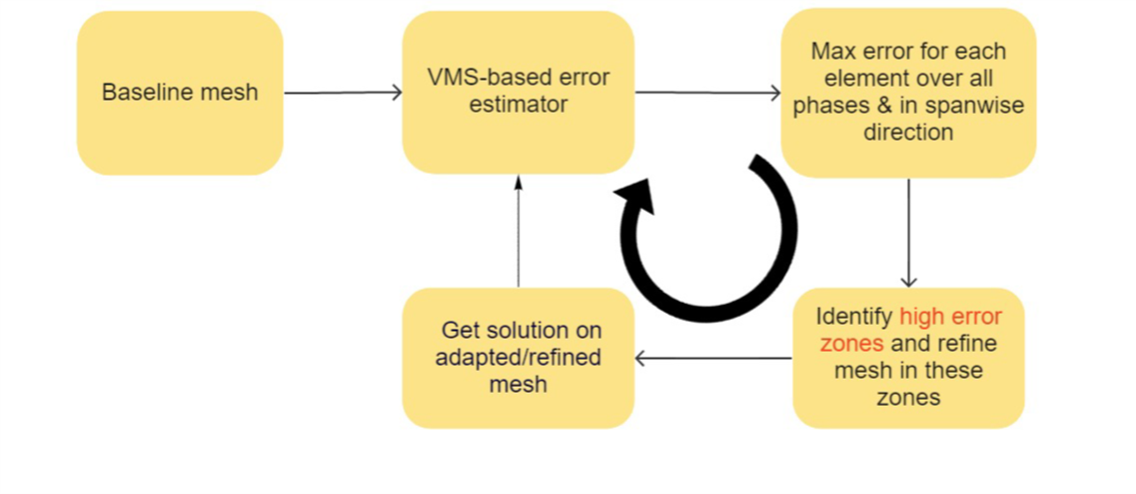
\includegraphics[width=1\textwidth]{figures/adapt_strat/zonal_based.png}
	\caption{Flowchart for zonal adaptation strategy}
	\label{fig:zonal_based_strat}
\end{figure}

For example, a sample of estimated error field in the case of flow over a surging airfoil is shown in Figure \ref{fig:zonal_based_strat_schematic}.
Note that maximum element-level error is obtained for all phases of the cycle and in spanwise direction.
Estimated error is higher in the wake region, as well as in the regions through which the leading edge vortex (LEV) traverses.
High error zones are identified in, and mesh in these zones is refined by a specified factor.

\begin{figure}[H]
	\centering
	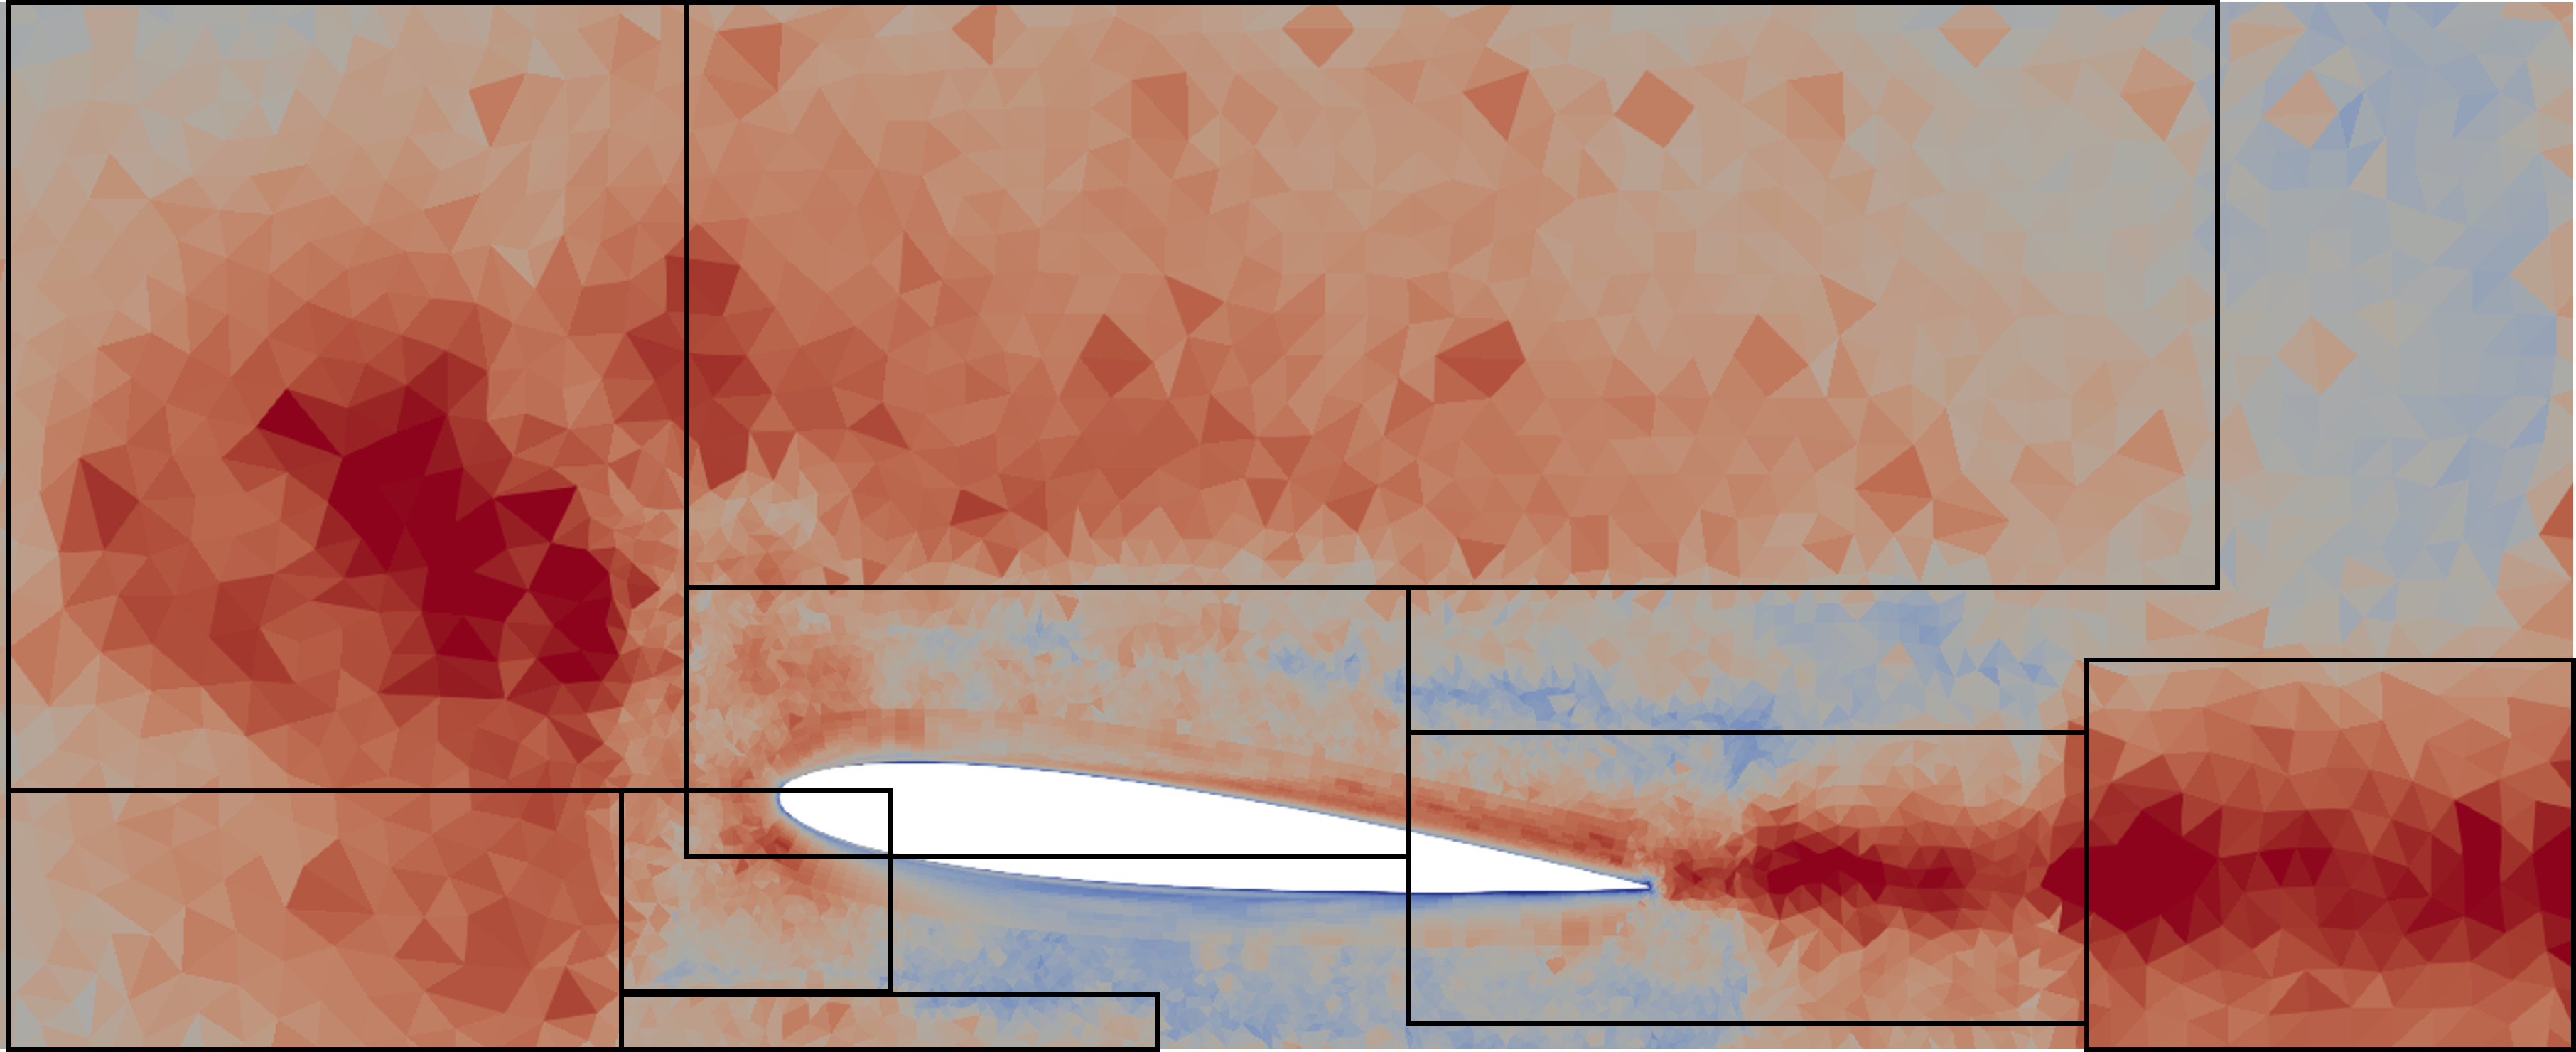
\includegraphics[width=0.75\textwidth]{figures/adapt_strat/zonal_based_schematic.png}
	\caption{Schematic of zonal refinement strategy}
	\label{fig:zonal_based_strat_schematic}
\end{figure}

\subsection{Nodal Size Field-based Adaptation}
\label{sec:sf_adapt}

The second strategy employs a fully automated mesh adaptation based on the VMS-based error estimator. In this strategy, the estimated error and a specified target error are used to compute the desired mesh size or resolution in a local fashion, i.e., at every mesh vertex. We refer to this as the nodal size field, and the mesh is refined or coarsened based on this nodal size field. 

In this adaptive strategy, the VMS-based error is calculated on the initial mesh. Based on the estimated error, a nodal size field is calculated using the following equation \cite{zhang19}

\begin{equation}
	\frac{e_k}{\tilde{e}_k} = \left(\frac{h_{old}}{h_{new}}\right)^{m+N/2} 
	\label{eq:diez}
\end{equation}

Here, $e_k$ is the measured local error (in the $\HOne$-seminorm) at an element $k$, $\tilde{e}_k$ is the local target error as specified by the user, $m$ is the polynomial order of the approximation space (i.e., $m=1$ for the linear finite elements used currently) , and $N$ is the number of spatial dimensions. $h_{old}$ is the current size of the element, and $h_{new}$ is the desired new mesh size.
This new mesh size at the element level is assembled at the node/vertex level to perform mesh adaptation.
The flowchart for this strategy is shown in Figure \ref{fig:size_based_strat}.

\begin{figure}[H]
	\centering
	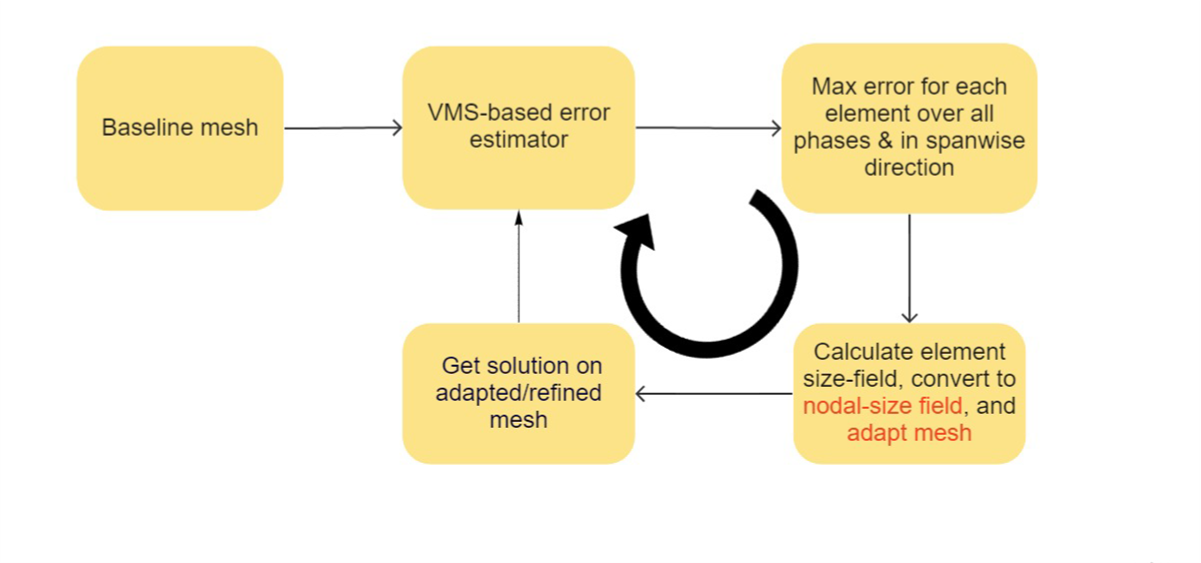
\includegraphics[width=1\textwidth]{figures/adapt_strat/size_based.png}
	\caption{Flowchart for nodal size field-based adaptation strategy}
	\label{fig:size_based_strat}
\end{figure}

\subsection{Feature-based Refinement/Adaptation}

The third strategy is to employ feature-based refinement/adaptation. 
This strategy allows for refinement around the dominant flow features and also along the path/trajectory of such features.
One of the primary flow features is the leading edge vortex (LEV) in the current problems of interest focused on surging airfoils. 
Figure \ref{fig:feature_based_strat_schematic} shows an example of the LEV path and size with respect to the airfoil. 
Mesh refinement is applied along this path as shown by the shaded region.


Two aspects are involved in this strategy: feature detection and tracking, and refinement/adaptation along the feature. These are discussed below.


	
\begin{figure}[H]
	\centering
	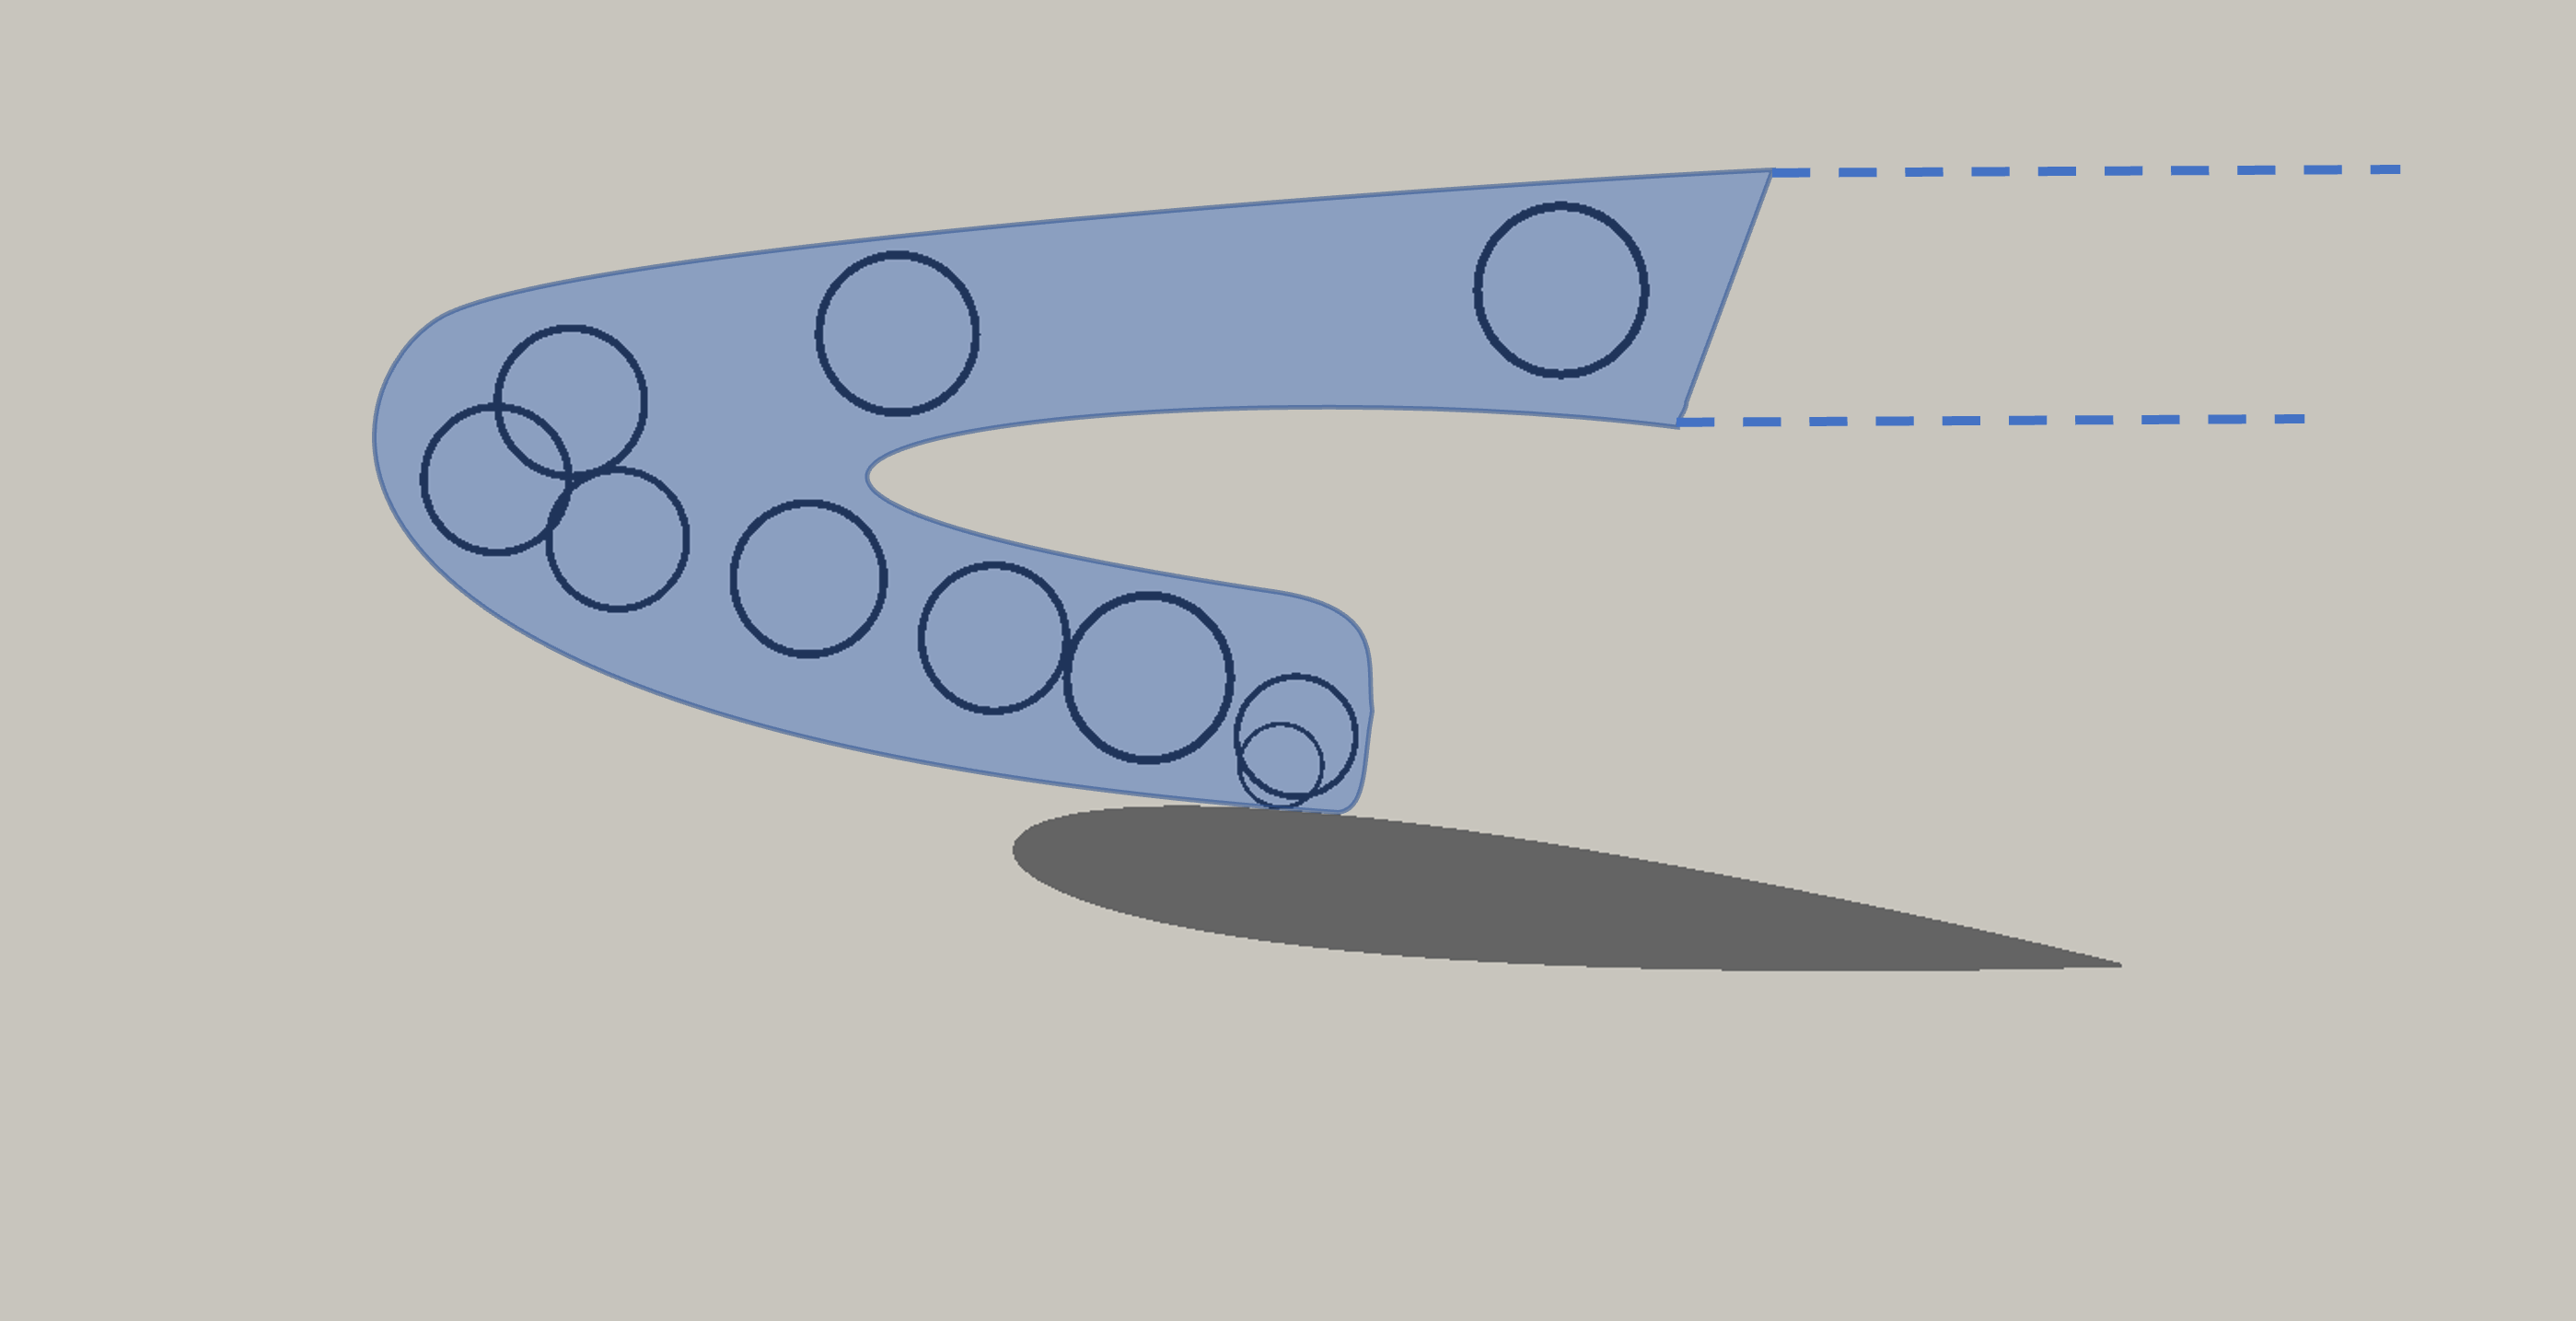
\includegraphics[width=0.75\textwidth]{figures/adapt_strat/feature_based_schematic.png}
	\caption{Schematic of feature-based refinement strategy}
	\label{fig:feature_based_strat_schematic}
\end{figure}

\subsubsection{LEV Detection and Tracking}
\label{sec:LEV_detect_track}

%TODO: Show pics and schematics from AIAA paper and presentations (LEV trace)

In this section, we quantify the evolution of the LEV based on its size and position.
In order to do so, phase- and spanwise-averaged data is obtained over multiple cycles.
Note that the LEV forms during the retreating portion of the surging cycle when the boundary layer separates and the separated shear layer rolls up into a vortex. Subsequently, this vortex separates/ejects from the airfoil, and advects with the background flow.
%For example, in Figure \ref{fig:LEV_tracking}, difference between the instantaneous and phase and span averaged vorticity is shown.
Thus, the phase of formation of the LEV is first detected and in subsequent phases the LEV is tracked.
Pressure and velocity data is analyzed to automatically detect the formation of the LEV.
In the retreating portion of the cycle, location with minimum pressure is determined starting at $\psi=180^\circ$.
The first phase at which the minimum pressure location is off the airfoil surface (i.e., away from the airfoil and into the flow) is tagged to be a potential phase for LEV formation.
At this potential phase, velocity profile is obtained over multiple lines passing through the minimum pressure location.
These are radial lines that are taken at an equispaced interval along the azimuth in the plane of the airfoil (note that the data is averaged in the spanwise direction).
These radial lines are shown in Figure \ref{fig:LEV_tracking2}.
Along these lines, at first a relative velocity is computed with respect to the velocity at the minimum pressure location.
Subsequently, normal component of the relative velocity is obtained (i.e., normal to each line), which is the azimuthal or tangential component in the polar coordinate system centered around the minimum pressure location.
The azimuthal component (of the relative velocity) is analyzed against the velocity profile of a Lamb-Oseen vortex.
It is noteworthy that the azimuthal component of the relative velocity along several radial lines at multiple phases in the surging cycle were visually analyzed for different cases and found to fit the Lamb-Oseen vortex model fairly well.

The trace of the LEV is then obtained by applying this process over multiple phases in the surging cycle, which can be used to quantify LEV evolution and to apply feature-based adaptation (as shown above in Figure \ref{fig:feature_based_strat_schematic}).

\begin{figure}[H]
	\begin{subfigure}{0.5\textwidth}
		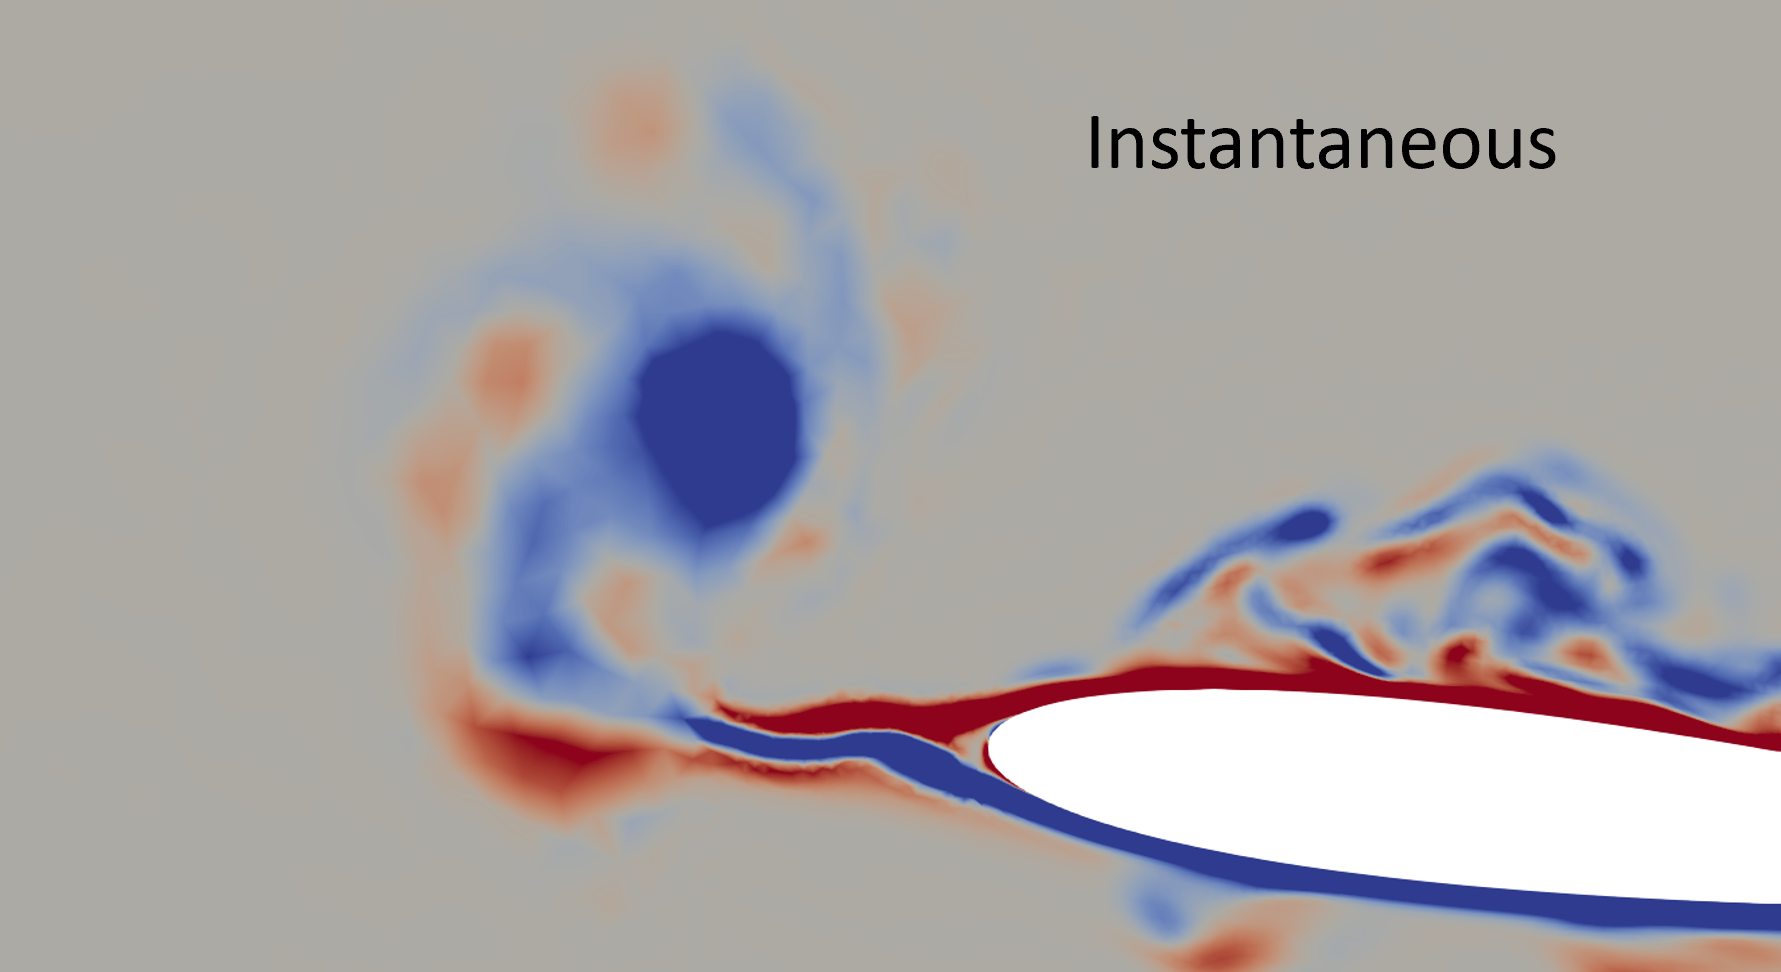
\includegraphics[width=1\textwidth]{figures/adapt_strat/LEV_tracking1.png}
		\caption{Instantaneous LEV}
		\label{fig:LEV_tracking1}
	\end{subfigure}
	\begin{subfigure}{0.51\textwidth}
	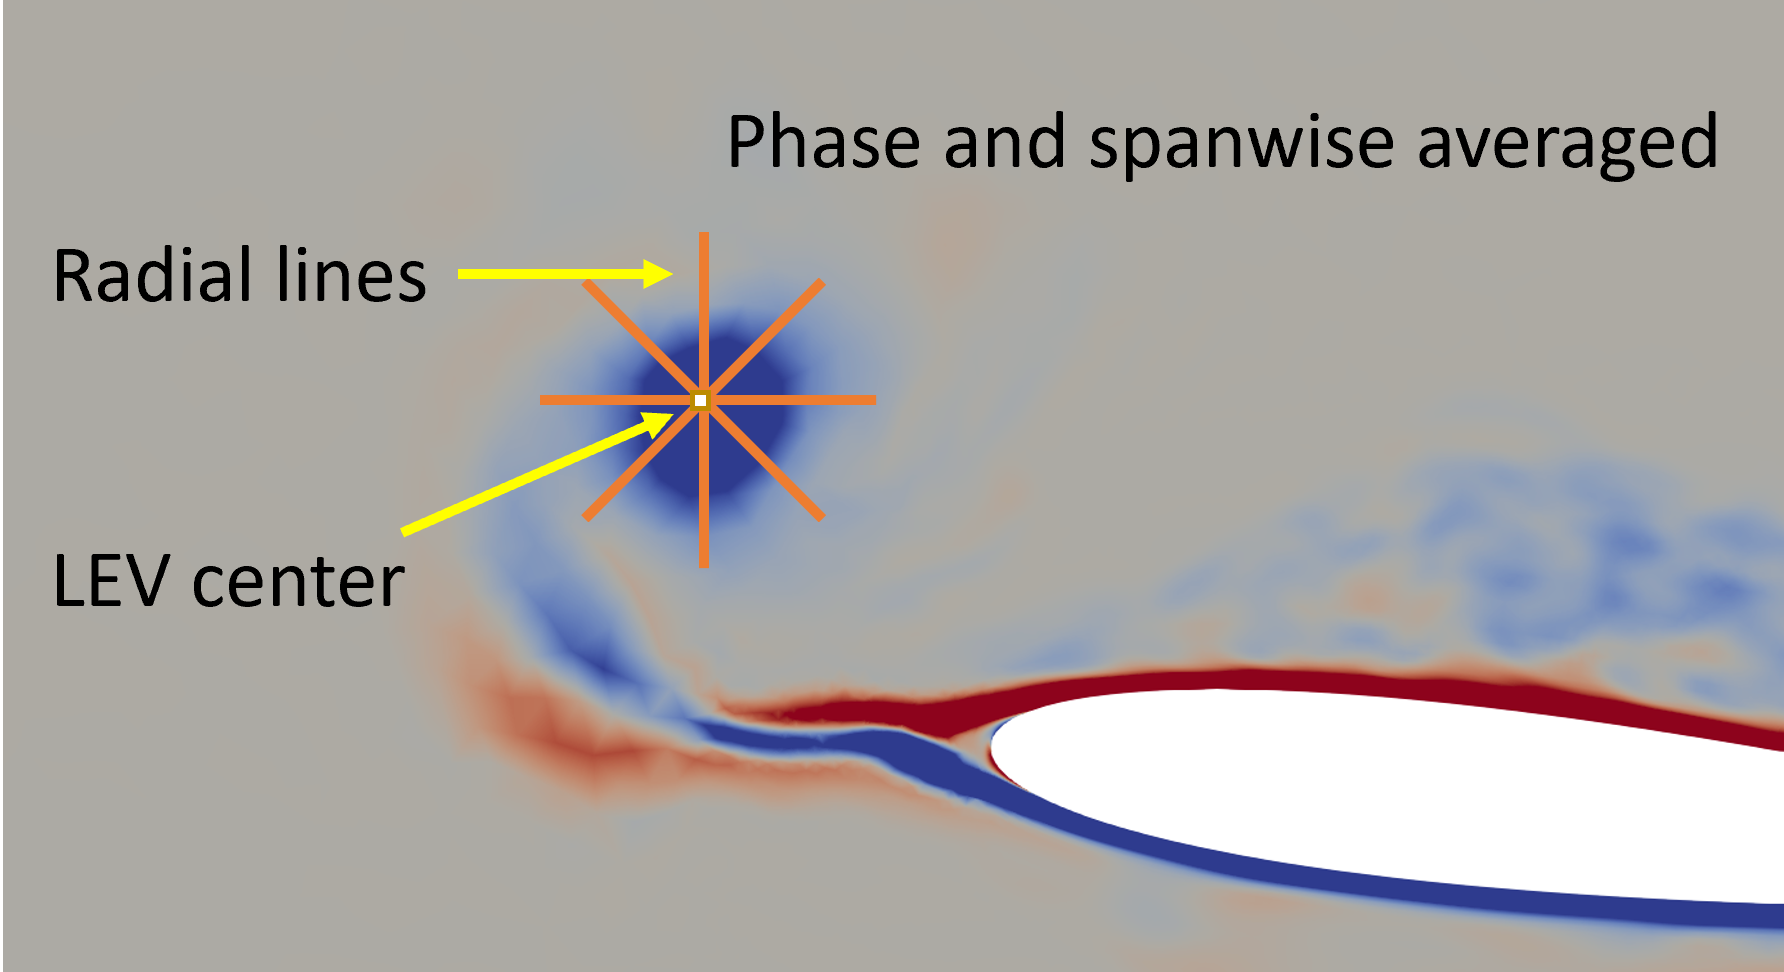
\includegraphics[width=1\textwidth]{figures/adapt_strat/LEV_tracking2.png}
	\caption{Averaged LEV}
	\label{fig:LEV_tracking2}
	\end{subfigure}

	\centering
	\begin{subfigure}{0.5\textwidth}
	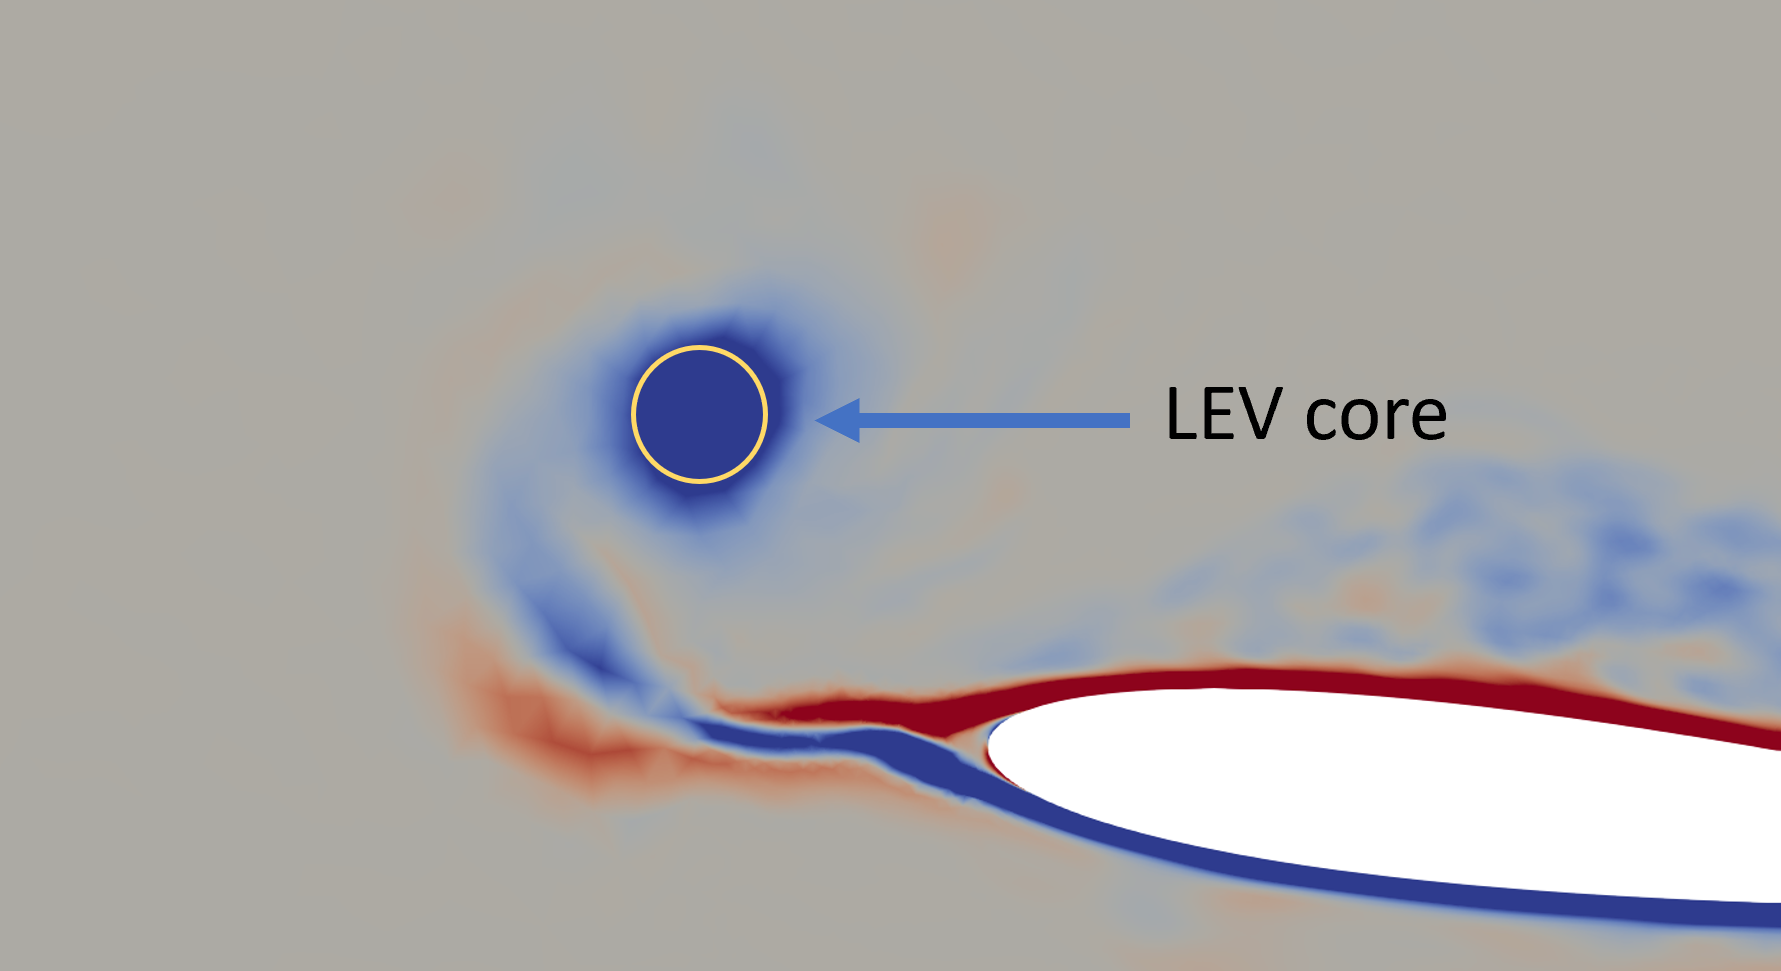
\includegraphics[width=1\textwidth]{figures/adapt_strat/LEV_tracking3.png}
	\label{fig:LEV_tracking3}
    \caption{Averaged LEV with core radius}
\end{subfigure}
	
	\caption{Schematic of LEV quantification}
	\label{fig:LEV_tracking}
\end{figure}


\subsubsection{LEV-based Refinement/Adaptation}

For a given simulation, we can follow three steps: (i) get information on the approximate path and extent that a certain feature will follow, (ii) estimate the error along this path/region, and (iii) perform refinement/adaptation along this path.
For example, in the case of flow over surging airfoils, the path and size of LEV over a surging cycle is used to detect portions in the mesh where refinement is applied.
Similarly, other features such as trailing edge vortex (TEV) can also be targeted using such a feature-based refinement. The flowchart for this strategy is shown in Figure \ref{fig:feature_based_strat}.

\begin{figure}[H]
	\centering
	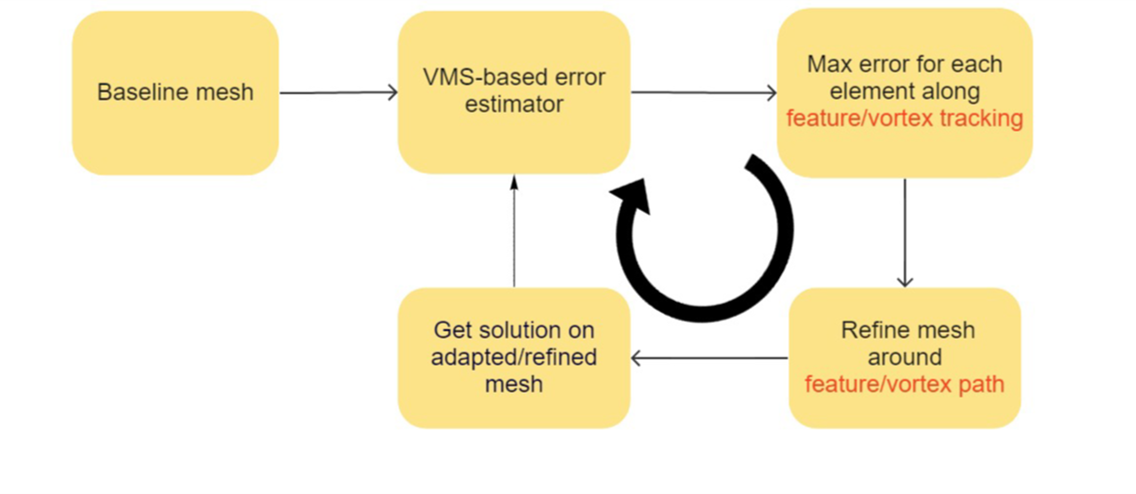
\includegraphics[width=1\textwidth]{figures/adapt_strat/feature_based.png}
	\caption{Flowchart for feature-based refinement strategy}
	\label{fig:feature_based_strat}
\end{figure}



\label{sec:adapt_strat_overview}
%\section{Non-dimensionalization of Error}

%One convenient aspect of the VMS approach to obtaining an error estimate is that the resulting units of the estimate are  



%%%xxx LATER Add a multi-D case (internal layer or boundary layer). Add a comment on Ainsworth 2013 paper with global effectivity order 60-100 for Pe of O(100).

